\scanpage{229}
\mspage{762}

point $1$ of $\mathbb U$, so that the universal covering of
$\mathbb S_0$ pointed over $e_0$
is identified with the exponential \unsure{covering}
\[
\tag{11}
\diagram{\begin{tikzcd}[ampersand replacement=\&,column sep=large,row sep=small]
\mathbb R \arrow[r] \& \mathbb U \&
(\xrightarrow{\sim}\mathbb S_0)\\
t \arrow[r,mapsto] \& \exp 2i\pi t \&
(\mapsto \mathbb R^+\exp 2i\pi t.
\end{tikzcd}}
\]

Thus, a lifting of $u_{\unsure{\mathbb S^1}}$
\inserted{to $\widetilde u$} amounts to the choice of $t\in\mathbb R$ such that
\[
\tag{12}
\exp 2i\pi t=\frac{u(1)}{|u(1)|}\qquad
\deleted{\unsure{\text{is written}}}
\]
i.e. to the choice of an argument $t$ of $u(1)$.

We apply the construction of $\widetilde G$ of $1^\circ)$
to the case of $G=\mathrm{Gl}(2,\mathbb R)^{\pm1}$,
we find an extension structure
\[
\tag{13}
\diagram{\begin{tikzcd}[ampersand replacement=\&,column sep=1.4em]
1\arrow[r]\&\mathbb Z\arrow[r]\&
\mathrm{Gl}(2,\mathbb R)^{\pm1\,\sim}\arrow[r]\&
\mathrm{Gl}(2,\mathbb R)^{\pm1}\arrow[r]\&1.
\end{tikzcd}}
\]

\deleted{\unsure{Propo}}\inserted{which induces}
over the identity component $\mathrm{Sl}(2,\mathbb R)$
of $\mathrm{Gl}(2,\mathbb R)^{\pm1}$ an extension structure
\[
\tag{14}
\diagram{\begin{tikzcd}[ampersand replacement=\&,column sep=1.5em]
1\arrow[r]\&\mathbb Z\arrow[r]\&
\mathrm{Sl}(2,\mathbb R)^{\sim}\arrow[r]\&
\mathrm{Sl}(2,\mathbb R)\arrow[r]\&1.
\end{tikzcd}}
\]

\begin{tabular}{|p{0.9\linewidth}}
\uline{Proposition} The group $\mathrm{Sl}(2,\mathbb R)^{\sim}$ is
$1$-connected, and even \deleted{\unsure{contra}}
homeomorphic to $\mathbb R^3$.
\end{tabular}

\margin{228}

\begin{center}
228\\
\texttt{https://grothendieck.umontpellier.fr}\\
Université de Montpellier, UMR CNRS 5149, Case courrier 051, Place Eugène Bataillon\\
34095 Montpellier cedex 5 - France
\end{center}

\scanpage{230}

\uline{Proof} Since the inclusion
\[
\tag{15}
\diagram{\begin{tikzcd}[ampersand replacement=\&,column sep=large]
\mathbb U\arrow[r,hook]\&\mathrm{Sl}(2,\mathbb R)
\end{tikzcd}}
\]
is a homotopy equivalence,
\deleted{\unsure{which}} is identified \inserted{topologically}
with the inclusion
$\diagram{\begin{tikzcd}[ampersand replacement=\&,column sep=large]
\mathbb U\arrow[r]\&\mathbb U\times\mathbb R^2
\end{tikzcd}}$,
we are reduced to proving that
\deleted{\unsure{over} $\mathbb U$}
\inserted{the inverse image $\mathbb U^{\sim}$}
of $\mathbb U$ in $\mathrm{Sl}(2,\mathbb R)^{\sim}$
is identified with the universal covering
$\deleted{\unsure{\mathbb R}}\,\mathbb R$ of $\mathbb U$
(pointed over $1$ by $0\ldots$)
Now if $u\in\mathbb U$, the \deleted{\unsure{last}}
choice of a $\widetilde u$ over $u$, i.e. of a lifting of
$\dfrac{u(1)}{|u(1)|}$ to $\mathbb R$ by formula (12),
is identified (since $\dfrac{u(1)}{|u(1)|}=u(1)=u$)
with the choice of a $t\in\mathbb R$ such that $\exp 2i\pi t\in u$, O.K.

\uline{Corollary 1} The \unsure{inverse} \unsure{subgroup} in
$\mathrm{Sl}(\unsure{2},\mathbb R)^{\sim}$ of a
finite cyclic subgroup \inserted{of order $n$} is $\simeq\mathbb Z$
($\exists!$ generator $\overline\omega$ of it,
such that we have $\overline\omega^{\,n}=\omega'_0$,
where $\omega'_0$ is the \deleted{\unsure{canonical}} generator
of the $\operatorname{Ker}(\mathrm{Sl}(2,\mathbb R)^{\sim}
\to\mathrm{Sl}(2,\mathbb R))$).

\margin{Applying this to the center
$\{\pm1\}$ of $\mathrm{Sl}(2,\mathbb R)$,
we find a canonical element $\omega_0\in\mathrm{Sl}(2,\mathbb R)^{\sim}$
with $\omega_0^2=\omega'_0$.}

\uline{Corollary 2} The action of a $g\in\mathrm{Gl}(2,\mathbb R)^{-1}$
on $\deleted{\unsure{\overline\omega}}\,\omega'_0$
(or on the center $\omega_0^{\mathbb Z}$ of
$\mathrm{Sl}(2,\mathbb R)^{\sim}$)
is via $\omega'_0\mapsto{\omega'_0}^{-1}$
(resp. $\omega_0\mapsto\omega_0^{-1}$) $\ldots$

\margin{229}

\begin{center}
229\\
\texttt{https://grothendieck.umontpellier.fr}\\
Université de Montpellier, UMR CNRS 5149, Case courrier 051, Place Eugène Bataillon\\
34095 Montpellier cedex 5 - France
\end{center}

\scanpage{231}
\mspage{763}

$3^\circ)$ \uline{The group} $\mathrm{Gl}(2,\mathbb Z)^{\sim}$.

Let $\mathrm{Gl}(2,\mathbb Z)^{\sim}$ be the inverse image of
$\mathrm{Gl}(2,\mathbb Z)$ in $\mathrm{Gl}(2,\mathbb R)^{\pm1\,\sim}$,
so that we have an extension structure
\[
\tag{16}
\diagram{\begin{tikzcd}[ampersand replacement=\&,column sep=1.2em,row sep=small]
1\arrow[r]\&\mathbb Z\arrow[r]\&\mathrm{Gl}(2,\mathbb Z)^{\sim}\arrow[r]\&
\mathrm{Gl}(2,\mathbb Z)\arrow[r]\&1.\\
\&\deleted{\unsure{n}}\arrow[u,mapsto]\arrow[r,mapsto]\&
\deleted{\unsure{\omega'_0}}\\
\&n\arrow[r,mapsto]\&\unsure{\omega_0^n|{\omega'_0}^{\,n}}
\end{tikzcd}}
\]

I would like to describe $\mathrm{Gl}(2,\mathbb Z)^{\sim}$ by generators
and relations. For this, I note this:

\begin{tabular}{|p{0.9\linewidth}}
\uline{Proposition} The inverse image
\inserted{in $\mathrm{Gl}(2,\mathbb Z)^{\sim}$}
of the cyclic subgroups $L_\rho\simeq\mathbb Z/6\mathbb Z$
and $L_\sigma\simeq\mathbb Z/4\mathbb Z$ generated by
$\rho$ and $\sigma$ are isomorphic to $\mathbb Z$.
\end{tabular}

This follows from the

\uline{Corollary} (to the proposition p. 762): For every
finite cyclic subgroup $\unsure{\mathfrak Z|\mathfrak z}\subset
\mathrm{Sl}(2,\mathbb R)$, the inverse image of
$\unsure{\mathfrak Z|\mathfrak z}$ in
$\mathrm{Sl}(2,\mathbb R)^{\sim}$ is isomorphic to $\mathbb Z$.

Indeed, by conjugation \unsure{we may assume} that
$\unsure{\mathfrak Z|\mathfrak z}\subset\mathbb U$,
i.e. $\unsure{\mathfrak Z|\mathfrak z}=\mu_n(\mathbb C)$,
but then $\unsure{\widetilde{\mathfrak Z}|\widetilde{\mathfrak z}}$
is identified with the set of $t\in\mathbb R$ with
$(\exp 2i\pi t)^n=1$ i.e. $\exp 2i\pi(nt)=1$ i.e.

\margin{230}

\begin{center}
230\\
\texttt{https://grothendieck.umontpellier.fr}\\
Université de Montpellier, UMR CNRS 5149, Case courrier 051, Place Eugène Bataillon\\
34095 Montpellier cedex 5 - France
\end{center}

\scanpage{232}

\[
t\in\frac1n\mathbb Z,
\]
the group of these $t$ is $\simeq\mathbb Z$, q.e.d.

\uline{Corollary} There exist
$\widetilde\rho\in\mathrm{Sl}(2,\mathbb Z)^{\sim}$ and
$\widetilde\sigma\in\mathrm{Sl}(2,\mathbb Z)^{\sim}$,
over $\rho$ and $\sigma$ respectively, such that we have
\[
\tag{17}
\widetilde\rho^{\,3}=\widetilde\sigma^{-2}
\]
\margin{for a more \unsure{pleasant} statement, see (20) below $\ldots$}
The set of these systems $(\widetilde\rho,\widetilde\sigma)$
is a torsor under $\mathbb Z$, by the operation
\[
\tag{18}
\diagram{\begin{tikzcd}[ampersand replacement=\&,column sep=large]
(\widetilde\rho,\widetilde\sigma)\arrow[r,mapsto]\&
(\widetilde\rho\,{\omega'_0}^{\,2n},
\widetilde\sigma\,{\omega'_0}^{\,3n}),
\end{tikzcd}}
\]
where $\omega'_0$ is the canonical generator of
$\diagram{\begin{tikzcd}[ampersand replacement=\&,]
\mathrm{Sl}(2,\mathbb Z)^{\sim}\arrow[r]\&
\mathrm{Sl}(2,\mathbb Z)
\end{tikzcd}}$.

We can also say that the inverse image of the element
$\deleted{\unsure{=-\mathrm{id}}}$
\inserted{of the center $\{\pm1\}$} of $\mathrm{Sl}(2,\mathbb Z)$
\deleted{\unsure{the unique}}
\deleted{(the central element \unsure{distinct from|$\ne$}
$+1$ of $\mathrm{Sl}(2,\mathbb Z)$)}
\deleted{is a torsor under $\mathbb Z$, and the choice}
\inserted{is a group isomorphic to $\mathbb Z$, with a}
unique generator $\omega_0$ satisfying
\deleted{\unsure{of a} lifting}
\[
\tag{19}
\begin{gathered}
\omega_0^2=\omega'_0
\quad(\inserted{\text{the}}\ \text{canonical generator of}\\
\diagram{\begin{tikzcd}[ampersand replacement=\&,]
\mathrm{Sl}(2,\mathbb Z)^{\sim}\arrow[r]\&
\mathrm{Sl}(2,\mathbb Z)
\end{tikzcd}})
\end{gathered}
\]

\margin{it \unsure{is} better to say: $\exists!$ generator
$\widetilde\rho$ \inserted{(resp. $\widetilde\sigma$)}
of the inverse image $\unsure{\widetilde L_\rho|L_\rho}$ of $L_\rho$
(resp. $L_\sigma$) in $\mathrm{Sl}(2,\mathbb Z)^{\sim}$,
over $\rho$ (resp. $\sigma$), and we then have relations (20)}

and this being so, it is possible to lift $\rho$ to $\widetilde\rho$,
\inserted{$\sigma$ to $\widetilde\sigma$} satisfying
\[
\tag{20}
\widetilde\rho^{\,3}=\omega_0^{-1},\qquad
\widetilde\sigma^{\,2}=\omega_0
\]
\margin{\uline{Do the verification}}
And this time, $\widetilde\rho$ and $\widetilde\sigma$
are uniquely deter-

\margin{231}

\begin{center}
231\\
\texttt{https://grothendieck.umontpellier.fr}\\
Université de Montpellier, UMR CNRS 5149, Case courrier 051, Place Eugène Bataillon\\
34095 Montpellier cedex 5 - France
\end{center}

\scanpage{233}
\mspage{764}

mined. This follows \deleted{\unsure{in a way}}
\inserted{\deleted{\unsure{from the}}}
at once from the preceding proposition.

\unsure{i)} Let us consider the inverse image of $\{1,\tau\}\subset\mathrm{Gl}(2,\mathbb Z)$
in $\mathrm{Gl}(2,\mathbb Z)^{\sim}$,
\deleted{\unsure{a group}} extension of
$\{1,\tau\}\simeq\mathbb Z/2\mathbb Z$ by $\mathbb Z$
--- I say that this extension is \uline{split}.

\margin{\uline{N.B.}
$\tau=\tau_\infty=\begin{pmatrix}-1&0\\0&1\end{pmatrix}$
i.e. $\tau(x+iy)=\unsure{-}x+iy$
(reflection with respect to the $y$-axis)}

Indeed, the action of $\tau$ on $\mathbb S_0$
lifts to the action of $\widetilde\tau$ \deleted{of}
of order $2$ on
$\deleted{\unsure{\mathbb R}}\,
\widetilde{\mathbb S}_0\simeq\mathbb R$,
which is given by
\[
\tag{21}
\widetilde\tau t=\frac12-t
\]
for we have for $z\in\mathbb U$, $z=\exp 2i\pi t$
\[
\tag{22}
\begin{aligned}
\tau z&=-\overline z=-\exp 2i\pi t
=\exp(\pi it-2i\pi t)\\
&=\exp\unsure{\{}\,2i\pi
\underbrace{\left(\frac12-t\right)}_{\widetilde\tau(t)}.
\end{aligned}
\]

\deleted{I} It is perhaps more convenient to work with
$\tau'=\tau'_\infty=\begin{pmatrix}0&1\\1&0\end{pmatrix}$,
which \deleted{is} exchanges $e_0=1$ and $e_1=i$,
i.e. the reflection \unsure{with respect|by} to the main diagonal.
This automorphism stabilizes $\mathbb U$, and fixes the point
$\exp\dfrac{\pi i}{\unsure{4|8}}=\dfrac{\sqrt2}{2}(i+1)\unsure{)}$,
it lifts to
\[
\tag{23}
\widetilde{\tau'}(t)=2i\pi\left(\frac1{\unsure{8|4}}-t\right).
\]
Let us note that \deleted{$\unsure{\widetilde{\tau'}|\tau'}$}
the action of $\widetilde{\tau'}$ (like that

\margin{232}

\begin{center}
232\\
\texttt{https://grothendieck.umontpellier.fr}\\
Université de Montpellier, UMR CNRS 5149, Case courrier 051, Place Eugène Bataillon\\
34095 Montpellier cedex 5 - France
\end{center}

\scanpage{234}

of $\widetilde\tau$) on $\omega_0$ is the symmetry $\omega_0\mapsto\omega_0^{-1}$ (cf. end of the preceding \S\ ). I say that we have
\[
\begin{array}{ll}
(24)&\widetilde\tau'(\widetilde\rho)=\widetilde\rho^{-1},\qquad
\widetilde\tau'(\widetilde\sigma)=\widetilde\sigma^{-1}.
\end{array}
\]
The formulas are \unsure{also|thus} written
\[
\widetilde\tau'(\widetilde\rho^{-1})=\widetilde\rho,\qquad
\widetilde\tau'(\widetilde\sigma^{-1})=\widetilde\sigma
\]
they are valid \deleted{\unsure{and}} in $\unsure{\mathrm{Sl}}(2,\mathbb Z)$, so to see that they are valid in $\mathrm{Sl}(2,\mathbb Z)^{\sim}$, it suffices to show that the left-hand \unsure{sides} satisfy the \unsure{characteristic} relations (20), which is written
\[
\widetilde\tau'\bigl(\underbrace{\widetilde\rho^{-3}}_{\omega_0^{\deleted{\unsure{-1}}}}\bigr)=\omega_0^{-1},\qquad
\widetilde\tau'\bigl(\underbrace{\widetilde\sigma^{-2}}_{\omega_0^{-1}}\bigr)=\omega_0
\]
i.e. $\widetilde\tau'(\omega_0)=\omega_0^{-1}$, OK.

\begin{tabular}{|l}
\uline{Theorem.} The group $\mathrm{Sl}(2,\mathbb Z)^{\sim}$ admits\\
the presentation (with two generators $\widetilde\rho,\widetilde\sigma$)\\[3pt]
$(25)\qquad\boxed{\widetilde\rho^3\cdot\widetilde\sigma^2=1}$
\end{tabular}

\uline{Proof} Let $\unsure{\Pi|\pi}$ be the group \deleted{\unsure{generated}} \inserted{defined} by this presentation, and let us consider the homomorphism
\diagram{
\begin{tikzcd}[ampersand replacement=\&,column sep=large,row sep=tiny]
\unsure{\Pi|\pi}\arrow[r] \& \mathrm{Sl}(2,\mathbb Z)/\pm1=\{\rho,\sigma\mid\rho^3=\sigma^2=1\}\\
(\widetilde\rho,\widetilde\sigma)\arrow[r,mapsto] \& (\rho,\sigma)\ \mathrm{mod}\{\pm1\}
\end{tikzcd}
\quad(26)
}

\margin{233}

\begin{center}
233\\
\texttt{https://grothendieck.umontpellier.fr}\\
Université de Montpellier, UMR CNRS 5149, Case courrier 051, Place Eugène Bataillon\\
34095 Montpellier cedex 5 - France
\end{center}

\scanpage{235}
\mspage{765}

the group $\mathrm{Sl}(2,\mathbb Z)/\pm1$ is identified with the quotient of $\unsure{\pi|\Pi}$ by the normal subgroup generated by the element $\uline{\omega_0}\overset{\mathrm{dfn}}{=}\widetilde\rho^{-3}=\widetilde\sigma^2$.
But this element being \unsure{central}, the group generated by $\uline{\omega_0}$ is already normal.
thus we have an exact sequence
\diagram{
$(27)\quad$
\begin{tikzcd}[ampersand replacement=\&,column sep=large,row sep=tiny]
n\arrow[r,mapsto] \& \uline{\omega_0}^{n} \& \& \\
\mathbb Z\arrow[r] \& \unsure{\Pi|\pi}\arrow[r] \& \mathrm{Sl}(2,\mathbb Z)/\pm1\arrow[r] \& 1
\end{tikzcd}
}
which maps into the exact sequence
\diagram{
\deleted{$\unsure{(28)|(27)}$}\quad
\begin{tikzcd}[ampersand replacement=\&,column sep=large,row sep=tiny]
1\arrow[r] \& \mathbb Z\arrow[r] \& \mathrm{Sl}(2,\mathbb Z)^{\sim}\arrow[r] \& \mathrm{Sl}(2,\mathbb Z)/\pm1\arrow[r] \&1\\
\& n\arrow[r,mapsto] \&\omega_0^{n}\&\&
\end{tikzcd}
}
inducing \inserted{identity} isomorphisms on the end factors --- thus by the lemma \unsure{of the|of} $5$
$\unsure{\pi|\Pi}\longrightarrow\mathrm{Sl}(2,\mathbb Z)^{\sim}$ is an isomorphism, q.e.d.

\begin{tabular}{|l}
\uline{Corollary 1} The group $\mathrm{Gl}(2,\mathbb Z)^{\sim}$ admits\\
the presentation (with three generators $\widetilde\rho,\widetilde\sigma,\widetilde\tau'$)
\end{tabular}
\[
\begin{array}{ll}
(28)&\boxed{
\widetilde\tau'{}^{2}=\deleted{\unsure{1,|\omega_0}}\,
\widetilde\rho^3\cdot\widetilde\sigma^2=1,\quad
\widetilde\tau'(\widetilde\rho)=\widetilde\rho^{-1},\quad
\widetilde\tau'(\widetilde\sigma)=\widetilde\sigma^{-1}}
\end{array}
\]

I am going to \unsure{try} to present the \deleted{\unsure{element}} \inserted{group}
$\mathrm{Gl}(2,\mathbb Z)^{\sim}$ \unsure{with|in} three involutive generators,
\deleted{\unsure{at the of}} $\widetilde r_0,\widetilde r_1,\widetilde r_\infty$ over the elements
$r_0,\unsure{r_1|\sigma_0},r_\infty$ of $\mathrm{Gl}(2,\mathbb Z)^{-}$, by \unsure{drawing inspiration} \unsure{from the formulary|from the formularies} of $\mathrm{Sl}(2,\mathbb Z)$:

\margin{234}

\begin{center}
234\\
\texttt{https://grothendieck.umontpellier.fr}\\
Université de Montpellier, UMR CNRS 5149, Case courrier 051, Place Eugène Bataillon\\
34095 Montpellier cedex 5 - France
\end{center}

\scanpage{236}

\[
\begin{array}{ll}
(29)&\left\{
\begin{aligned}
r_\infty&=\tau_\infty=\begin{pmatrix}-1&0\\0&1\end{pmatrix}\\
r_0&=\tau'_\infty=\begin{pmatrix}0&1\\1&0\end{pmatrix}\\
r_1&=-\tau'_0=\begin{pmatrix}-1&1\\0&1\end{pmatrix}
\end{aligned}
\right.
\end{array}
\]
\margin{$\left[\begin{array}{ll}
(30)&\left\{
\begin{aligned}
r_0(\rho)&=\rho^{-1},\quad r_0(\sigma)=\sigma^{-1}\\
r_1&=\rho^{-1}r_0=r_0\rho\\
r_\infty&=\sigma r_0=r_0\sigma^{-1}
\end{aligned}\right.
\end{array}\right.$}

Note that $(\widetilde\rho,\widetilde\tau')$ \unsure{generate} a group isomorphic to $D_\infty$, which I denote by $D_{\widetilde\rho}$,
likewise $(\widetilde\sigma,\widetilde\tau')$ \unsure{generates|generate} a group $D_{\widetilde\sigma}$,
isomorphic to $D_\infty$. Finally $(\omega_0,\widetilde\tau')$ \unsure{generate} a group $D_{\omega_0}$, again isomorphic to $D_\infty$. We have a diagram
\diagram{
$(31)\quad$
\begin{tikzcd}[ampersand replacement=\&,column sep=large,row sep=large]
\&D_{\omega_0}\arrow[dl,"i"']\arrow[dr,"j"]\&\\
D_{\widetilde\rho}\&\&D_{\unsure{\widetilde\sigma|\widetilde\rho}}
\end{tikzcd}
\qquad
$\begin{aligned}
&\left\{\begin{aligned}
i(\omega_0)&=\widetilde\rho^{-3}\\
i(\widetilde\tau')&=\widetilde\tau'
\end{aligned}\right.\\[4pt]
&\left\{\begin{aligned}
j(\omega_0)&=\widetilde\sigma^2\\
j(\unsure{\widetilde\tau'})&=\widetilde\tau'
\end{aligned}\right.
\end{aligned}$
}
and corollary 1 is written in the form
\[
\begin{array}{ll}
(32)&\mathrm{Gl}(2,\mathbb Z)^{\sim}\simeq D_{\widetilde\rho}*_{D_{\omega_0}}D_{\widetilde\sigma}
\end{array}
\]
(amalgamated \unsure{sum} of groups).

Now we can take in $D_{\widetilde\rho},D_{\widetilde\sigma}$ the involutive generators
\[
\begin{array}{ll}
(33)&\left\{\begin{array}{lll}
\widetilde r_0=\widetilde\tau'=\widetilde\tau'_\infty&\text{and}&
\widetilde r_1\overset{\mathrm{dfn}}{=}\widetilde\rho^{-1}\widetilde r_0=\widetilde r_0\widetilde\rho\quad\text{in }D_{\widetilde\rho}\\
\widetilde r_0=\cdots\cdots&\text{and}&
\widetilde r_\infty\overset{\mathrm{dfn}}{=}\unsure{\widetilde\sigma\,\widetilde r_0}=\widetilde r_0\widetilde\sigma^{-1}
\end{array}\right.
\end{array}
\]

\margin{235}

\begin{center}
235\\
\texttt{https://grothendieck.umontpellier.fr}\\
Université de Montpellier, UMR CNRS 5149, Case courrier 051, Place Eugène Bataillon\\
34095 Montpellier cedex 5 - France
\end{center}

\scanpage{237}
\mspage{766}

and we then find

\uline{Corollary 2} $\mathrm{Gl}(2,\mathbb Z)^{\sim}$ admits a presentation (with three involutive generators $\widetilde r_0,\widetilde r_1,\widetilde r_\infty$):
\[
\begin{array}{ll}
(34)&\boxed{\widetilde r_0^2=\widetilde r_1^2=\widetilde r_\infty^2=1,\quad
\Bigl(\underbrace{\widetilde r_0^{\deleted{\unsure{-1}}}\widetilde r_1}_{\widetilde\rho}\Bigr)^3
\overset{\deleted{\unsure{=}}}{\cdot}
\Bigl(\underbrace{\widetilde r_\infty\widetilde r_0^{\deleted{\unsure{-1}}}}_{\widetilde\sigma}\Bigr)^2=1}\\[-2pt]
&\hspace{13em}\deleted{\underbrace{\hspace{9em}}_{\unsure{\omega_0}}}
\end{array}
\]

\margin{236}

\begin{center}
236\\
\texttt{https://grothendieck.umontpellier.fr}\\
Université de Montpellier, UMR CNRS 5149, Case courrier 051, Place Eugène Bataillon\\
34095 Montpellier cedex 5 - France
\end{center}

\scanpage{238}

$4^\circ)$ \uline{The isomorphism} $\mathrm{Gl}(2,\mathbb Z)^{\sim}\simeq S\mathcal T_{1,1}$

\margin{$\unsure{\checkmark}$}
Put
\[
\begin{array}{ll}
(35)&\deleted{\unsure{X_1}}\quad X_1=\mathbb R^2/\mathbb Z^2\simeq(\mathbb R/\mathbb Z)^2\simeq\mathbb U\times\mathbb U.
\end{array}
\]
(model surface of genus $1$), write its composition law additively, and let
\[
\begin{array}{ll}
(36)&a_{1,0}=0\in X_1,\quad X_1\setminus\{a_{1,0}\}=X_1\setminus\{0\}=U_{1,1},
\end{array}
\]
model surface of type $(g,\nu)=(1,1)$.

The group $\mathrm{Gl}(2,\mathbb Z)$ is identified with the group of automorphisms of the topological group $X_1$, and thus operates on $X_1$ leaving fixed the origin $\deleted{a_{1,0}}\ 0$, hence it operates on $U_{1,0}$, whence a homomorphism
\diagram{
$(37)\quad$
\begin{tikzcd}[ampersand replacement=\&,column sep=large,row sep=tiny]
\mathrm{Gl}(2,\mathbb Z)\arrow[r,"\sim"]\&\mathcal T_{1,1}=\mathcal T(\unsure{U_{1,1}})\\
\&\begin{gathered}\text{group of isotopy classes}\\
\text{of homeomorphisms}\\
\text{of }U_{1,1},\end{gathered}
\end{tikzcd}
}
which we know to be an isomorphism. Moreover, $G=\mathrm{Gl}(2,\mathbb Z)$ operates \unsure{differentiably|differentially} on $\deleted{\unsure{\mathcal T|\tau}}\ X_1$, and the action on the \uline{tangent} space is identified with the tautological action of $\mathrm{Gl}(2,\mathbb Z)\subset\mathrm{Gl}(2,\mathbb R)$ on $\mathbb R^2$. Thus the group denoted by $\widetilde G$ in

\margin{237}

\begin{center}
237\\
\texttt{https://grothendieck.umontpellier.fr}\\
Université de Montpellier, UMR CNRS 5149, Case courrier 051, Place Eugène Bataillon\\
34095 Montpellier cedex 5 - France
\end{center}

\scanpage{239}
\mspage{767}

\unsure{$1^\circ$)} \unsure{e} is canonically isomorphic, as an extension of $G$ by $T_0=\mathbb Z$ (N.B. $\mathbb R^2$ and its quotient $X_1$ are canonically oriented) to the group $\mathrm{Gl}(2,\mathbb Z)^\sim$ \unsure{of} $3^\circ$.

Thus we find \deleted{the \unsure{Theorem}} \inserted{(cf. proposition p. 761)} the

\uline{Theorem} The inverse image under the isomorphism (37) of the extension $S\deleted{\unsure{*}}\mathcal T_{1,1}$ of $\mathcal T_{1,1}$ by $\mathbb Z$ is canonically identified with $\mathrm{Gl}(2,\mathbb Z)^\sim$, so it admits the \inserted{two} explicit presentations \unsure{of} $3^\circ$
\[
\begin{aligned}
\text{a)}\quad &
\underset{\deleted{\unsure{\omega\widetilde\sigma}}}{\widetilde\rho^{3}\cdot\widetilde\sigma^{2}}
=\underset{\deleted{\unsure{\omega_0}}}{1},\quad
\unsure{\widetilde\tau'}(\widetilde\rho)=\widetilde\rho^{-1},\quad
\widetilde\tau'(\widetilde\sigma)=\widetilde\sigma^{-1},\quad
\widetilde\tau'^{\,2}=1
\\[1ex]
\text{b)}\quad &
\widetilde r_0^{2}=\widetilde r_1^{2}=\widetilde r_\infty^{2}=1,\quad
\underset{\deleted{\unsure{\omega_0}}}{
(\widetilde r_0^{\deleted{\unsure{-1}}}\widetilde r_1)^3\cdot
(\widetilde r_\infty\widetilde r_0)^2}=1.
\end{aligned}
\]

Let us now interpret $\mathcal T_{1,1}$ and $S\mathcal T_{1,1}$ in terms of the fundamental group of $U_{1,1}$, which we \unsure{shall compute} by choosing (judiciously ?) a base point $a_{1,1}$ in $U_{1,1}$,
\[
\text{(38)}\qquad
\Pi_{1,1}\overset{\mathrm{dfn}}=\pi_1(U_{1,1},a_{1,1}),
\]
\[
\text{(39)}\qquad
\mathcal T_{1,1}\simeq\mathrm{Aut\,ext}_{\mathrm{lac}}(\Pi_{1,1})
\]
\margin{238}

\begin{center}
238\\
\texttt{https://grothendieck.umontpellier.fr}\\
Université de Montpellier, UMR CNRS 5149, Case courrier 051, Place Eugène Bataillon\\
34095 Montpellier cedex 5 - France
\end{center}

\scanpage{240}

\margin{\unsure{I use} the \unsure{notation} $\ell'_0$ instead of $\ell_0$, since $\ell_0$ already denotes a well-determined element of $\mathrm{Gl}(2,\mathbb Z)$ !}

We have a presentation of $\Pi_{1,1}$ by
\[
\text{(40)}\qquad
\Pi_{1,1}=\{x,y,\ell'_0\mid [x,y]\ell'_0=1\}
\]
and denoting by $L$ the subgroup\inserted{\unsure{-loops}} of $\Pi_{1,1}$ generated by $\ell'_0$, we shall have
\[
\text{(41)}\qquad
S\mathcal T_{1,1}\simeq
\mathrm{Norm}_{\mathrm{Aut}_{\mathrm{lac}}(\Pi_{1,1})}(L).
\]

Thus we should make explicit the action
\deleted{\unsure{of} $\unsure{S}$}
\diagram{\begin{tikzcd}[ampersand replacement=\&,column sep=large]
S\mathcal T_{1,1}\simeq\mathrm{Gl}(2,\mathbb Z)^\sim
\arrow[r] \& \mathrm{Aut}_{\mathrm{lac}}(\Pi_{1,1}),
\end{tikzcd}}
by the action of the generators $\widetilde\rho,\widetilde\sigma,\widetilde\tau'$ or $\widetilde r_0=\widetilde\tau',\widetilde r_1,\widetilde r_\infty$ --- action which must \unsure{normalize} $L$, and more precisely, transform $\ell'_0$ into $\ell'_0$ (for $\widetilde\rho,\widetilde\sigma$) or into $\ell_0'^{-1}$ (for $\widetilde\tau'=\widetilde r_0,\widetilde r_1,\widetilde r_\infty$). Thus we must make explicit the action of the generators on $x$ and on $y$. (N.B. $\Pi_{1,1}$ is the free group having as generators $x$ and $y$ \unsure{!})

Let us consider the principal covering $U_{1,1}^{\prime\,\unsure{a}}$ with group $\mathbb Z^2$ of $U_{1,1}=X_1-\{0\}$, induced by the principal \unsure{covering} $\mathbb R^2$ of $X_1=\mathbb R^2/\mathbb Z^2$, --- the inverse image of $U_{1,1}$ is $\mathbb R^2\setminus\mathbb Z^2$. Let us choose a base point \deleted{$\unsure{a}$}
\margin{239}

\begin{center}
239\\
\texttt{https://grothendieck.umontpellier.fr}\\
Université de Montpellier, UMR CNRS 5149, Case courrier 051, Place Eugène Bataillon\\
34095 Montpellier cedex 5 - France
\end{center}

\scanpage{241}
\mspage{768}

\deleted{\unsure{(44)|(42)}}
\[
a\in\mathbb R^2\setminus\mathbb Z^2,
\]
\unsure{up} above $a_{1,1}$, we will thus have a canonical isomorphism
\[
\text{(42)}\qquad
\Pi_{1,1}\simeq\pi_1(\mathbb R^2\setminus\mathbb Z^2,\mathbb Z^2;a)
\]
whence an exact sequence
\diagram{\begin{tikzcd}[ampersand replacement=\&,column sep=small,row sep=small]
\text{(43)}\quad \& 1\arrow[r] \&
\pi_1(\mathbb R^2\setminus\mathbb Z^2)\arrow[r] \&
\Pi_{1,1}\arrow[r]\arrow[d,equal] \&
\mathbb Z^2\arrow[r]\arrow[d,phantom,"\simeq"{description,rotate=90}] \& 1.\\
\&\&\&\pi_1(U_{1,1}=X_1\setminus\{a_{1,0}\}) \&
\pi_1(X_1)\arrow[d,phantom,"\simeq"{description,rotate=90}] \&\\
\&\&\&\& (\Pi_{1,1})_{\mathrm{ab}} \&
\end{tikzcd}}

The elements of the mixed $\pi_1$ are made explicit by Jean Malgoire's calculation using the pairs
\[
\text{(44)}\qquad
(\gamma,\ell)\qquad
\left(\begin{gathered}
\gamma\in\mathbb Z^2,\quad \ell\ \text{\unsure{class} of paths in}\\
\mathbb R^2\setminus\mathbb Z^2\ \text{from }a\text{ to }\deleted{\unsure{\gamma|\tau}}a+\gamma
\end{gathered}\right)
\]
which we ``\unsure{compose} like functions''.

\inserted{We will take, over the generators}
\deleted{Let us consider the}
$e_0,e_1$ of $\mathbb Z^2$, the elements $x,y$ defined by the straight-line paths from $a$ to $a+e_0$, resp. $a+e_1$, starting from the origin
\[
\text{(45)}\qquad
 a=\widetilde a_{1,1}=\left(+\frac12,+\frac12\right)
\]

\figure{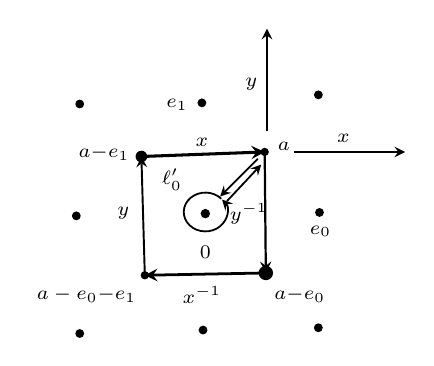
\begin{tikzpicture}[x=1.45cm,y=1.45cm,>=stealth,font=\scriptsize]
\fill (-1.10,0.96) circle (1.6pt);
\fill (-0.03,0.97) circle (1.6pt);
\fill (0.99,1.04) circle (1.6pt);
\fill (-1.13,-0.02) circle (1.6pt);
\fill (0,0) circle (1.7pt);
\fill (1.00,0.01) circle (1.6pt);
\fill (-1.10,-1.05) circle (1.6pt);
\fill (-0.02,-1.02) circle (1.6pt);
\fill (0.99,-1.00) circle (1.6pt);
\node[left] at (-0.07,0.95) {$e_1$};
\node[below] at (1.01,-0.02) {$e_0$};
\node[below] at (0,-0.20) {$0$};
\coordinate (a) at (0.52,0.54);
\coordinate (b) at (-0.56,0.50);
\coordinate (c) at (-0.53,-0.54);
\coordinate (d) at (0.53,-0.52);
\fill (a) circle (1.5pt);
\fill (b) circle (2.1pt);
\fill (c) circle (1.5pt);
\fill (d) circle (2.6pt);
\draw[->,line width=1.1pt] (b) -- (a);
\node[above] at (-0.03,0.50) {$x$};
\draw[->,line width=.7pt] (c) -- (b);
\node[left] at (-0.58,0.00) {$y$};
\draw[->,line width=1.0pt] (d) -- (c);
\node[below] at (-0.03,-0.55) {$x^{-1}$};
\draw[->,line width=.8pt] (a) -- (d);
\node at (0.38,0.00) {$y^{-1}$};
\draw[->,line width=.7pt] (0.54,0.72) -- (0.54,1.62);
\node[left] at (0.54,1.13) {$y$};
\draw[->,line width=.7pt] (0.78,0.54) -- (1.75,0.54);
\node[above] at (1.21,0.54) {$x$};
\node[right] at (0.55,0.59) {$a$};
\node[left] at (-0.58,0.53) {$a\unsure{-}e_1$};
\node[below left] at (-0.52,-0.56) {$a-e_0\unsure{-}e_1$};
\node[below right] at (0.52,-0.56) {$a\unsure{-}e_0$};
\draw[->,line width=.65pt] (0.46,0.48) -- (0.13,0.15);
\draw[->,line width=.65pt] (0.19,0.11) -- (0.49,0.43);
\draw[->,line width=.65pt] (0.14,0.13)
 arc[start angle=43,end angle=400,x radius=.19,y radius=.17];
\node[above left] at (-0.12,0.12) {$\ell'_0$};
\end{tikzpicture}}

Then the element $xyx^{-1}y^{-1}$ is represented by the path above, which is visibly opposite to the positively oriented ``straight-line'' loop from $a$ around the origin $0$.
\margin{240}

\begin{center}
240\\
\texttt{https://grothendieck.umontpellier.fr}\\
Université de Montpellier, UMR CNRS 5149, Case courrier 051, Place Eugène Bataillon\\
34095 Montpellier cedex 5 - France
\end{center}

\scanpage{242}

$5^\circ$) \uline{Digression on the} \inserted{\uline{coverings of}} \uline{germs of spaces.}

\margin{A) \uline{Coverings of germs}}
\margin{here we exclude \deleted{\unsure{the}} \inserted{not the} improper filter $(\varnothing\in\Phi)$ corresponding to the \uline{empty} germ of spaces}

A ``germ of spaces'' is defined by a topological space $S$ and a \deleted{base of a} filter $\Phi$ on $S$, a morphism from $(S,\Phi)$ to $(S',\Phi')$ is an element of
\[
\text{(46)}\qquad
\varinjlim_{S_i\in\Phi}\operatorname{Hom}_{\Phi_{\unsure{S_i|S'_i}},\Phi'}(S_i,S'),
\]
where \deleted{$\Phi_{S_i}$ is} for $S_i\in\Phi$, $\Phi_{S_i}$ is the filter induced by $\Phi$ on $S_i$, and $\operatorname{Hom}_{\Phi_{S_i},\Phi'}$ denotes the set of continuous maps \inserted{$f$} from $S_i$ to $S'$ compatible with $\Phi_{S_i},\Phi'$, i.e. such that $\forall S'_j\in\Phi'$, \deleted{$\unsure{f}$} we have $f^{-1}(S'_j)\in\Phi_{S_i}$. The composition of morphisms of germs is obvious.

A \uline{covering} (étale) of a germ $(S,\Phi)$ of topological spaces is an object of the category
\[
\text{(47)}\qquad
\underline{\mathrm{Rev}}(S,\Phi)=\varinjlim_{S_i\in\Phi}\underline{\mathrm{Rev}}(S_i);\qquad\unsure{*}
\]
\unsure{these|the} coverings form a category, which we could \inserted{probably} interpret \inserted{(at least in ``good cases'')} as the category of coverings of a suitable topos (namely the projective limit topos
\margin{241}

\begin{center}
241\\
\texttt{https://grothendieck.umontpellier.fr}\\
Université de Montpellier, UMR CNRS 5149, Case courrier 051, Place Eugène Bataillon\\
34095 Montpellier cedex 5 - France
\end{center}

\scanpage{243}
\mspage{769}

\margin{this \unsure{has been} done by Olivier Leroy?}

of the \inserted{(small)} étale topoi of the $S_i\in\Phi$).

This category, ``in the good cases'', tends to be multi-Galois, or even Galois.

We say that a germ \deleted{\unsure{is}} of spaces is $1$-connected, or simply connected, if the natural functor

\diagram{\begin{tikzcd}[ampersand replacement=\&,column sep=large,row sep=small]
{(48)} \& (\mathrm{Ens}) \arrow[r] \& \underline{\mathrm{Rev}}(S,\Phi) \\
 \& E \arrow[r,mapsto] \& {\unsure{{}^{1}\!E_{(S,\Phi)}|\widetilde E_{(S,\Phi)}},\ \text{constant covering with}} \\
 \& \& {\text{value }\unsure{E|\Phi}}
\end{tikzcd}}

is an equivalence of categories. This means that

$1^\circ)$ This functor is fully faithful (we say that $(S,\Phi)$ is $0$-connected), which means, if $S$ is locally connected, that $\forall S_i\in\Phi$, $\exists S_j\in\Phi$, $S_j\subset S_i$, such that \inserted{$S_j\ne\varnothing$ and} $(\pi_0(S_j)\longrightarrow\pi_0(S_i))$ is a constant map

\margin{thus this implies that this germ of spaces is nonempty}

$2^\circ)$ the functor is moreover \unsure{essentially!|essentially$^{\mathrm t}$} surjective, which means that for every $S_i\in\Phi$, $\exists S_j\in\Phi$, \inserted{$S_j\subset S_i$} such that for every connected component $S_{j,\alpha}$ of $S_j$, the outer homomorphism $\pi_1(S_{j,\alpha})\longrightarrow\pi_1(S_i)$ is trivial.

Coverings of germs of spaces form a fibered category over that

\margin{242}

\begin{center}
242\\
\texttt{https://grothendieck.umontpellier.fr}\\
Université de Montpellier, UMR CNRS 5149, Case courrier 051, Place Eugène Bataillon\\
34095 Montpellier cedex 5 - France
\end{center}

\scanpage{244}

of germs of spaces. The category of topological spaces \deleted{\illegible{1}} can be regarded as a full subcategory of that of germs of topological spaces by \unsure{associating} to every space $\unsure{S}$, the germ $(S,\Phi)$, where $\Phi$ is the trivial filter on $S$. This being so, the fibered category of coverings of germs of spaces \unsure{induces|induced} that of coverings of topological spaces.

Let $\deleted{\unsure{\mathcal S}}\mathcal X$ be a germ of spaces such that $\underline{\mathrm{Rev}}\mathcal X$ is a \inserted{multi-}Galois category, \deleted{Then} and let $\mathcal S$ be a $1$-connected germ of spaces, $\mathcal S\longrightarrow\mathcal X$ a morphism. Then we have

\diagram{\begin{tikzcd}[ampersand replacement=\&,column sep=large]
{(49)} \& \underline{\mathrm{Rev}}(\mathcal X) \arrow[r] \& \underline{\mathrm{Rev}}(\mathcal S) \& (\mathrm{Ens}) \arrow[l,"\sim"']
\end{tikzcd}}

fiber functor on $\underline{\mathrm{Rev}}(\mathcal X)$, which makes it possible to define
\[
(50)\qquad \pi_1(\deleted{\unsure{\mathcal S}}\unsure{\mathcal X},\mathcal S)
\]
as the $\pi_1$ relative to this fiber functor. If $\mathcal X$ is $0$-connected so $\underline{\mathrm{Rev}}(\mathcal X)$ is Galois, we will thus have, if $\Pi\simeq\pi_1(\mathcal X,\mathcal S)$, an equivalence of categories

\margin{243}

\begin{center}
243\\
\texttt{https://grothendieck.umontpellier.fr}\\
Université de Montpellier, UMR CNRS 5149, Case courrier 051, Place Eugène Bataillon\\
34095 Montpellier cedex 5 - France
\end{center}

\scanpage{245}
\mspage{770}

\[
(51)\qquad \underline{\mathrm{Rev}}(\mathcal X)\simeq\mathrm{Ens}(\Pi).
\]

The group $\pi_1(\mathcal X,\mathcal S)$ depends functorially on the triple $(\mathcal S,\mathcal X,\mathcal S\longrightarrow\mathcal X)$ i.e. on the arrow $\mathcal S\longrightarrow\mathcal X$ in the category of germs of spaces, where $\deleted{\mathcal S}$ the source $\mathcal S$ is $1$-connected.

\unsure{Let|Let} $X$ be a topological space, $Y$ a subset of $X$, we \uline{call the germ of} $X$ \uline{around} $Y$ the germ of spaces $(X,\Phi)$, where $\Phi$ is the filter of neighborhoods of $Y$ \unsure{in|in} $X$, \uline{the residual germ of $X$ around $Y$} the germ of spaces $(X\setminus Y,\Phi_{X\setminus Y})$ induced on $X-Y$ (it is empty iff $Y$ is open).

\margin{We have a \unsure{diagram} of \unsure{canonical} morphisms
\diagram{\begin{tikzcd}[ampersand replacement=\&,column sep=large,row sep=large]
\unsure{\mathrm{Germ}_{Y}(X)} \arrow[d,hook] \& \unsure{\mathrm{Gerres}_{Y}(X)} \arrow[l,hook'] \arrow[d,hook] \\
X \& X-Y \arrow[l,hook']
\end{tikzcd}}\quad (52)}

We will use this notion \deleted{\unsure{especially}} in the case where $Y=\{x\}$, speaking also of the germ and residual germ of $X$ at $x$. (\uline{N.B.} the germ of $X$ at $x$ is always \deleted{\unsure{simp}} $1$-connected, but not the residual germ). Every germ of spaces \inserted{$(S,\Phi)$} can be interpreted as the residual germ of a space \deleted{$(\unsure{S},\unsure{\Phi})$} $\unsure{X}=S\cup\{\omega\}$ at a suitable point $\omega$ \ldots

\margin{244}

\begin{center}
244\\
\texttt{https://grothendieck.umontpellier.fr}\\
Université de Montpellier, UMR CNRS 5149, Case courrier 051, Place Eugène Bataillon\\
34095 Montpellier cedex 5 - France
\end{center}

\scanpage{246}

\unsure{.} I am interested in the case where $x\in X$ has a neighborhood homeomorphic to $\mathbb R^2$ --- i.e. $X$ is a surface at $x$. I will denote by $\deleted{D_{X,x}^{*}}$
\[
(53)\qquad D_{X,x}^{*}\quad\text{or}\quad D_x^{*}
\]
the residual germ of $X$ at $x$ (contained in the germ $D_{X,x}$ or $D_x$ of $X$ at $x$).

I am interested in the choice of a \uline{universal covering} $D_x^{*\,\sim}$ of $D_x^{*}$ --- but for \unsure{which|whom} I have to make a digression on the abstract notion of \uline{universal covering of a germ of spaces}.

Let $(S,\Phi)$ be a germ of spaces. A covering of $(S,\Phi)$ comes from a covering $S'_i$ of an $S_i\in\Phi$, and defines a germ of spaces $(S'_i,\Phi_{S'_i})$, where $\Phi_{S'_i}$ denotes the inverse image of $\Phi_{\deleted{\unsure{S'_i}}S_i}$ in $S'_i$. This germ of spaces \inserted{over $\mathcal S=(S,\Phi)$} (up to unique isomorphism of germs) does not depend on the choice of $S_i$, $S'_i$, but only on the element of $\underline{\mathrm{Rev}}(\mathcal S)$. We thus find a canonical functor

\margin{245}

\begin{center}
245\\
\texttt{https://grothendieck.umontpellier.fr}\\
Université de Montpellier, UMR CNRS 5149, Case courrier 051, Place Eugène Bataillon\\
34095 Montpellier cedex 5 - France
\end{center}

\scanpage{247}
\mspage{771}

\diagram{\begin{tikzcd}[ampersand replacement=\&,column sep=large]
{(54)} \& \underline{\mathrm{Rev}}(\mathcal S) \arrow[r] \& {(\unsure{\mathrm{Germesp}})/\mathcal S}
\end{tikzcd}}

which is \uline{fully faithful}. A germ of spaces $\mathcal S'$ over $\mathcal S$ is called \deleted{\unsure{the}} an \uline{étale covering} \uline{of} $\mathcal S$, if it is in the essential image. Thus the category $\underline{\mathrm{Rev}}(\mathcal S)$ of étale coverings of the germ of spaces $\mathcal S$ is equivalent to the full subcategory of the \deleted{\unsure{g}} category of germs of spaces, over the germ $\mathcal S$, \deleted{which} formed by the étale coverings of the said germ $\mathcal S$.

Let us assume \deleted{that} \unsure{always|always} that the category $\underline{\mathrm{Rev}}(\mathcal S)$ is \deleted{\unsure{g}} multi-Galois. The $1$-connected objects are called universal coverings of $\mathcal S$ --- \deleted{if $\underline{\mathrm{Rev}}(\mathcal S)$ is Galois,} they form a groupoid, connected iff $\underline{\mathrm{Rev}}(\mathcal S)$ is Galois i.e. iff the germ $\mathcal S$ is $0$-connected. The universal \unsure{coverings!|coverings} of $\mathcal S$ can be interpreted as germs of spaces. Let $\widetilde{\mathcal S}$ be such a universal covering, then $\widetilde{\mathcal S}$ is indeed a \unsure{$1$-connected|$1$. connected} germ of spaces, and $\widetilde{\mathcal S}\longrightarrow\mathcal S$ makes it possible to define $\pi_1(\mathcal S,\widetilde{\mathcal S})$. This being so, we have a canonical isomorphism
\[
(55)\qquad \pi_1(\mathcal S,\widetilde{\mathcal S})\simeq\mathrm{Aut}_{\underline{\mathrm{Rev}}(\mathcal S)}(\widetilde{\mathcal S})
\]

\margin{Which expresses that $\pi_1(\mathcal S,\widetilde{\mathcal S})$ is none other than the $\pi_1$ of the ``abstract'' \inserted{multi-}Galois category $\underline{\mathrm{Rev}}(\mathcal S)$, ``calculated'' at the $1$-connected element $\widetilde{\mathcal S}$.}

\margin{\figure{\begin{tikzpicture}[x=1cm,y=1cm]
\draw (0,0) -- (0.18,0.43);
\draw (0.04,0.10) -- (0.14,0);
\end{tikzpicture}}}

\margin{246}

\begin{center}
246\\
\texttt{https://grothendieck.umontpellier.fr}\\
Université de Montpellier, UMR CNRS 5149, Case courrier 051, Place Eugène Bataillon\\
34095 Montpellier cedex 5 - France
\end{center}
